\chapter{Analysis}
\section{Introduction}
This chapter will present the analysis of the 2 systems presented in Chapter 6 and 7. Also we will take the better system according to our needs and present the modified system according to our system.
\section{OpenID Based pseudonym System}
\begin{figure}[h]
	\centering
	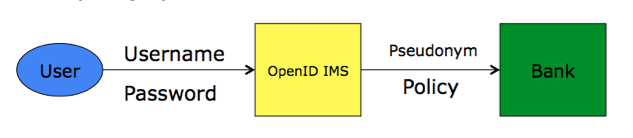
\includegraphics[width=\textwidth]{figures/OpenID}
	\caption{Pseudonym System with OpenID IMS}
	\label{fig:OpenID}
\end{figure}
With the use of OpenID IMS we add a pseudonymous layer in the system. This provides us the necessary privacy. But in order to do so OpenID provider needs access to a lot of data. Some of the example data is:
\begin{itemize}
\item UserID
\item Account ID 
\item Policies	
\end{itemize}
In addition to that, the provider needs to store the mapping database from UserID to Pseudonym. Bank really has to trust the provider with storage of all this sensitive data. In some cases bank might not want the provider to store such data by themselves.
\\
\\In case there is a discrepancy, the authorities need to go both to the bank to get the transaction data as well as the provider for the mapping data.
\section{IDEMIX Based pseudonym System}
\begin{figure}[h]
	\centering
	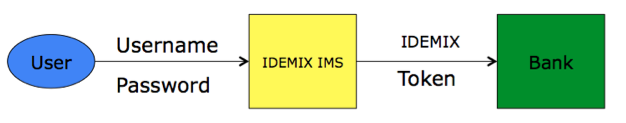
\includegraphics[width=\textwidth]{figures/IDEMIX}
	\caption{Pseudonym System with IDEMIX IMS}
	\label{fig:IDEMIX}
\end{figure}
With the use of IDEMIX IMS we add a pseudonymous layer in the system. This provides us the necessary privacy. In order to do so, IDEMIX IMS just need to store the IDEMIX credential of the user. 
\\
\\The provider doesn’t need to store any mapping database on his side. It is easier for bank to implement, as bank really doesn’t have to trust the IDEMIX IMS to store sensitive data.
\\
\\In case there is a discrepancy, the authorities need to go only to the bank to get the transaction data as well as the mapping data from the IDEMIX tokens.
\section {IDEMIX implementation in the Real World}
From above 2 analyses, we conclude that IDEMIX implementation of pseudonymous system is more favorable to bank than the OpenID implementation. 
\\Now we will try to fit this implementation in our system, which includes Nykredit as the Bank, Signicat as the 3rd party, DTU as corporate customer and other government institutions as authorities.
\subsection{Addition of the New User}
Addition of the new user can happen as following:
\begin{enumerate}
	\item DTU registers the new user with the Nykredit giving them the user details and policies that should apply to the particular user regarding the account. 
	\begin{enumerate}
		\item Nykredit registers this new user with his User ID with the IMS system
	\end{enumerate}
	\item Nykredit issue an IDEMIX policy credential for the given user to DTU. This credential contains the policy information and account information for the user.
	\item DTU then use this policy credential to register the new user with Signicat. 
	\begin{enumerate}
		\item Signicat inquire about the user data with the authorities
		\item Authorities verify the user data to Signicat
	\end{enumerate}
	\item After that Signicat issue final IDEMIX credential for the IMS system. This credential is then used to create pseudonym IDEMIX tokens for the user. 
\end{enumerate}
\begin{figure}[h]
	\centering
	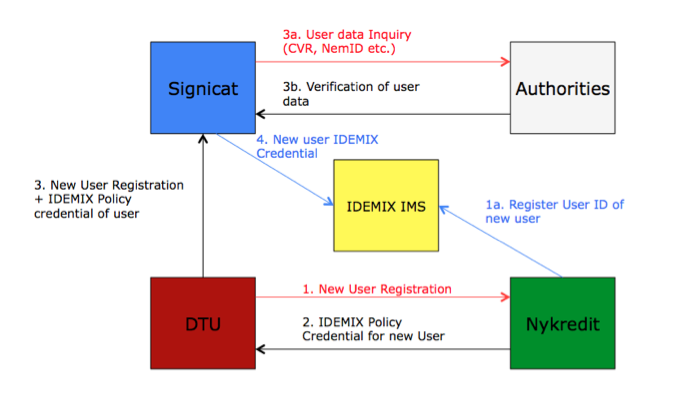
\includegraphics[width=\textwidth]{figures/Real}
	\caption{IDEMIX Credential issuance for a new user}
	\label{fig:Real}
\end{figure}
\begin{figure}[h]
	\centering
	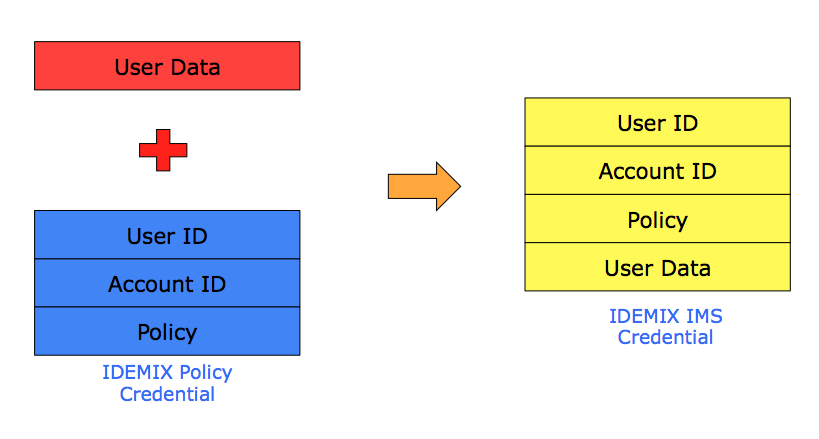
\includegraphics[width=\textwidth]{figures/Final}
	\caption{Final IDEMIX Credential from Policy Credential}
	\label{fig:Final}
\end{figure}
\FloatBarrier
\subsection{Addition of a New Customer}
Addition of the new customer is almost same as addition of new user:
\begin{enumerate}
	\item An administrator goes to Nykredit to open a bank account on behalf of DTU 
	\begin{enumerate}
		\item Nykredit registers DTU as new customer in their internal system.
		\item Nykredit register the DTU administrator with his User ID with the IMS system
	\end{enumerate}
	\item Nykredit issue an IDEMIX policy credential for the  DTU administrator to himself. This credential contains the policy information and account information for the administrator.
	\item Administrator then use this policy credential to register himslef as owner of the new DTU account with Signicat. 
	\begin{enumerate}
		\item Signicat inquire about the data given in the credential with the authorities
		\item Authorities verify the dta to Signicat
	\end{enumerate}
	\item After that Signicat issue final IDEMIX credential for the IMS system. This credential is then used to create pseudonym IDEMIX tokens for the administrator. 
\end{enumerate}
\subsection{Technical Requirements}
In this system DTU as a client doesn't need to change anything on their side to be a customer at Nykredit. All the system for DTU is web based where they can just add/remove users and also DTU users login to the system using the browser.
\\
\\Nykredit have to implement IDEMIX issuer service on their side to issue IDEMIX Policy credential. This is done so that Nykredit doesn’t have to store the sensitive data at the 3rd party. Use of this credential ensures that this data remains safe. Nykredit also have to implement IDEMIX verifier service to verify the user identity.
\\
\\Signicat have to implement IDEMIX issuer service also to issue final IDEMIX credentials.
\\\\
IMS have to implement IDEMIX user service to create the IDEMIX tokens for the user while user is logging in.
\section{Summary}
In this chapter we analyzed 2 different pseudonym systems as discusses in chapter 6 and 7. Also after that we discussed in detail the implementation of the IDEMIX system in the real world in our system.
